\documentclass[aspectratio=169]{beamer}

% Custom theme and packages
\usepackage{beamertheme-custom}
% Custom symbols and commands
\usepackage{symbols-custom}

\graphicspath{{figures/}}

\title{Accumulator models of response time}
\author{Joachim Vandekerckhove}
\date{Spring 2025}

% Font
\usefonttheme[onlymath]{serif}

\begin{document}

\maketitle

\begin{frame}[fragile]{Process models of speeded choice response time}
Accumulator models describe the process that generates speeded CRTs\\[2ex]\pause

These models start from a number of representation assumptions:
\bi
\i Deciders accumulates small bits of evidence, sequentially over time, from the stimulus they were exposed to
\i Most stimuli are at least somewhat ambiguous (noisy)
\i Deciders aggregates this evidence with the evidence already accumulated
\i After each accumulation step, deciders evaluate whether the total amount of information in favor of a decision is enough to execute a response
\ei

\end{frame}

\begin{frame}[fragile]{Process models of speeded choice response time}
There exist many accumulator models for response times\\[2ex]\pause

They differ in, among other things:
\bi
\i Whether they allow for two, many, or only one choice
\i Whether time is treated as discrete or continuous
\i Whether the accumulation of evidence is at a constant rate
\i Whether the evidence `leaks' over time
\i Whether evidence for one choice counts as evidence against the other
\i ...
\ei

\end{frame}


\begin{frame}[fragile]{Process models of speeded choice response time}
Evidence is accumulated over short periods of time
\begin{figure}[htp]
\centering
{\includegraphics[scale=0.80,bb=0 0 400 180,clip]{walk.eps}}
\end{figure}

\end{frame}


\begin{frame}[fragile]{Process models of speeded choice response time}
The evidence accumulation process occurs at each trial of an experiment, with each process hitting one or the other boundary at some time point
\begin{figure}[htp]
\centering
{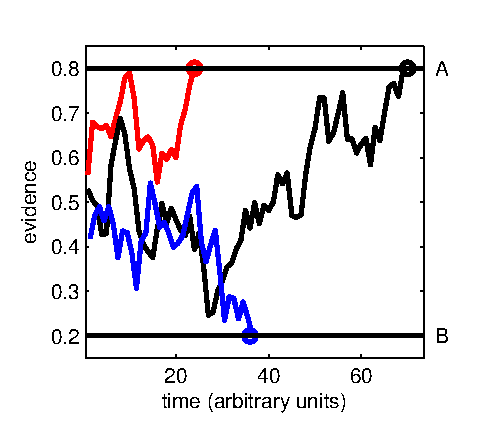
\includegraphics[scale=0.80]{choice.eps}}
\end{figure}
The boundaries represent distinct choice options
\end{frame}


\begin{frame}[fragile]{Process models of speeded choice response time}
On repeated runs, the \emph{first passage times} can form a smooth distribution
\begin{figure}[htp]
\centering\vspace{-2ex}
{\includegraphics[scale=0.66]{rdmpmeth.eps}}
\end{figure}
This distribution is sometimes called the \emph{Wiener distribution}:
$$p(t, a) = W(\delta,\alpha,\tau,\beta)$$
\end{frame}

\definecolor{verylightgray}{rgb}{.9,.9,.9}

\begin{frame}[fragile]{Diffusion models for two-choice response times}

Cognitive models that use assumptions like these are usually called \emph{accumulator models}\pause

A particularly popular case of this category of models are the \emph{diffusion models} for two-choice response times\pause

Diffusion models are popular for a few reasons: they are mathematically somewhat convenient, they seem to fit data well in practice, and they have a small number of easy-to-interpret parameters

\end{frame}


\begin{frame}[fragile]{Diffusion models for two-choice response times}\centering
\begin{tabular}{cll}
\rowcolor{black}
           & {\it\color{white}parameter} &  {\it\color{white}interpretation} \\
\rowcolor{verylightgray}
$\delta$   &  drift rate              &  dominance ($\eta$, $d'$) \\
\rowcolor{lightgray}
$\alpha$   &  boundary separation     &  caution \\
\rowcolor{verylightgray}
$\tau$     &  nondecision time        &  time for encoding and responding \\
\rowcolor{lightgray}
$\beta$    &  initial bias            &  a priori response bias \\
\end{tabular}

\begin{figure}[htp]
\centering\vspace{-2ex}
{\includegraphics[scale=0.66]{rdmpmeth.eps}}
\end{figure}
\end{frame}



\begin{frame}[fragile]{Diffusion model parameters in delta plots}

Diffusion model parameter effects become tell-tale patterns in delta plots\\[4ex]

 \centering
\begin{tabular}{cll}
\rowcolor{black}
           & {\it\color{white}parameter} &  {\it\color{white}interpretation} \\
\rowcolor{verylightgray}
$\delta$   &  drift rate              &  dominance ($\eta$, $d'$) \\
\rowcolor{lightgray}
$\alpha$   &  boundary separation     &  caution \\
\rowcolor{verylightgray}
$\tau$     &  nondecision time        &  time for encoding and responding
\end{tabular}

\begin{figure}[htp]
\centering\vspace{-2ex}
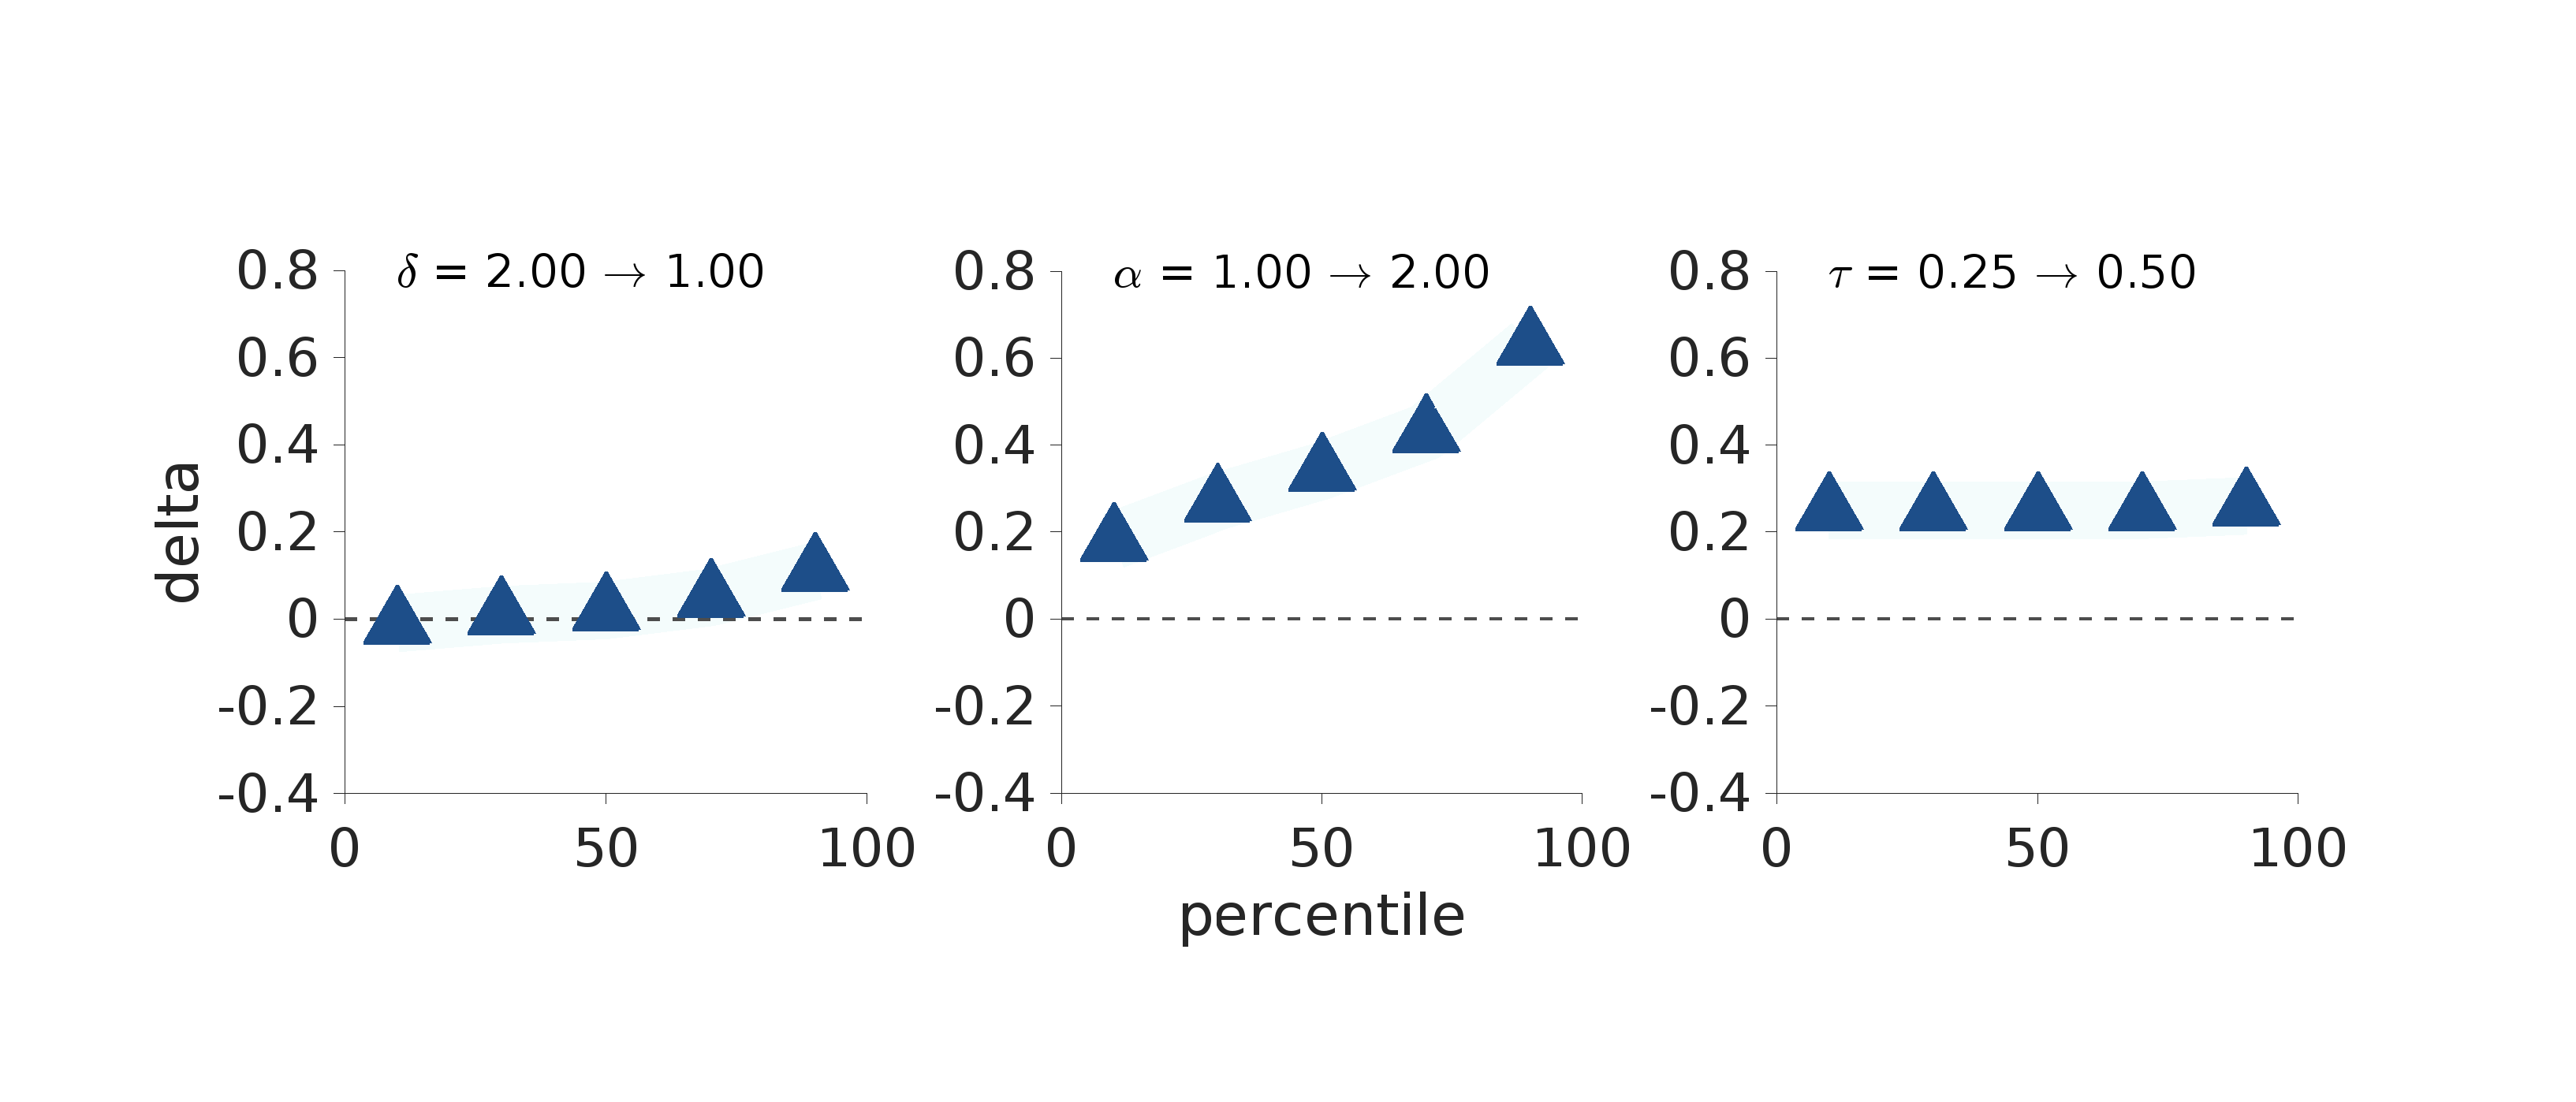
\includegraphics[scale=0.20,bb= 0 0 1552 600,clip]{deltadiff.eps}
\end{figure}

\end{frame}



\begin{frame}[fragile]{Diffusion model parameters in delta plots}

Effects on the initial bias often only show when you split the delta plot by error/correct --- they can cancel out if you don't!\\[4ex]

 \centering
\begin{minipage}{.35\textwidth}
\begin{tabular}{ll}
\cellcolor{black}         {\it\color{white}parameter}      \\ 
\cellcolor{verylightgray} $\beta$, initial bias  \\
\cellcolor{black}         {\it\color{white}interpretation} \\ 
\cellcolor{verylightgray} a priori response bias  \\
\end{tabular}
\end{minipage}
\begin{minipage}{.6\textwidth}
\begin{figure}[htp]
\centering

\includegraphics[scale=0.30,bb=550 100 1000 500,clip]{deltadiffbias.eps}
\end{figure}
\end{minipage}

\end{frame}



\begin{frame}[fragile]{Diffusion model parameter estimation}

While a quick look at delta plots can be informative, ultimately we want to estimate model parameters from data\\[2ex]\pause

Often, we will perform \emph{constrained parameter estimation} so that, for example each participant has one $\alpha_p$ and $\tau_p$, independent of condition\\[3ex]\pause

 \centering
\begin{minipage}{.58\textwidth}
\begin{tabular}{|cccc|}
\rowcolor{black}
{\it\color{white}person $p$} & {\it\color{white}condition $c$} & {\it\color{white}RT} & {\it\color{white}accuracy}       \\ 
1 & 3 & 0.71 & correct \\
1 & 5 & 0.49 & correct \\
$\vdots$ & $\vdots$ & $\vdots$ & $\vdots$ \\
1 & 3 & 0.43 & error \\
2 & 4 & 0.67 & error \\
$\vdots$ & $\vdots$ & $\vdots$ & $\vdots$ \\
9 & 2 & 0.61 & correct \\
9 & 2 & 0.39 & error \\\hline
\end{tabular}
\end{minipage} $\;\;\;\;\rightarrow\;\;$
\begin{minipage}{.3\textwidth}
\begin{tabular}{|ccc|}
\rowcolor{black}
{\it\color{white}$\alpha_p$} & {\it\color{white}$\delta_{pc}$} & {\it\color{white}$\tau_p$}       \\ 
1.61 & 0.45 & 0.24   \\
1.61 & 1.17 & 0.24   \\
$\vdots$ & $\vdots$ & $\vdots$ \\
1.61 & 0.53 & 0.24   \\
2.14 & 0.08 & 0.31   \\
$\vdots$ & $\vdots$ & $\vdots$ \\
1.41 & 0.79 & 0.27   \\
1.41 & 0.79 & 0.27   \\\hline
\end{tabular}
\end{minipage}

\end{frame}



\begin{frame}[fragile]{Weekly assignment: Generate delta plots for diffusion models}

Recreate the delta plots in the slides
\begin{itemize}
\item Using the \texttt{3-ddm/src/diffusion\_simulator.py} script to generate data from a diffusion model, write your own script to generate delta plots
\item Use as baseline parameters:
\begin{itemize}
\item $\delta = 2.00$ (and as contrast use $\delta = 1.00$)
\item $\alpha = 1.00$ (and as contrast use $\alpha = 2.00$)
\item $\tau = 0.25$ (and as contrast use $\tau = 0.50$)
\item $\beta = 0.35$ (and as contrast use $\beta = 0.65$)
\end{itemize}
\item Select a reasonable number of samples for the simulation
\item Use percentiles 10, 30, 50, 70, and 90
\item Make sure you label your axes, annotate the plot, and feel free to use pretty (readable!) colors
\end{itemize}

\end{frame}

%\begin{frame}[allowframebreaks]{References}
%\bibliographystyle{apacite}
%\bibliography{../cogs110B}
%\end{frame}


\maketitle

\end{document}
